\chapter{Křivočaré systémy souřadnic}

Kartézský systém souřadnic není jediný možný. Z~důvodu geometrie těles nebo symetrie problému může být v~praxi výhodné využít křivočarý systém souřadnic. Také je možné jej využít pokud kartézský systém nelze zavést protože prostor je zakřivený, například v~teorii relativity. Tím se zde však nebudeme zabývat, budeme předpokládat, že prostor je Euklidovský a~křivočarý systém souřadnic zavedeme transformací do kartézského. Mezi často používané křivočaré systémy souřadnic patří polární, cylindrický, sférický a~teorie obsáhne samozřejmě i~kartézský systém souřadnic.

Předpokládejme, že máme prostor \(E_n\), ve kterém máme kartézský systém souřadnic s~body určenými souřadnicemi \(P' = [P'_1, P'_2, ..., P'_n]\). Chceme zavést jiný systém souřadnic s~body určenými souřadnicemi \(P = [P_1, P_2, ..., P_n]\). Transformaci mezi souřadnými systémy popisuje sada funkcí \(p_i\):

\begin{equation}
P'_i = p'_i(P_1, P_2, ..., P_n)
\end{equation}

Opačná transformace pak je:

\begin{equation}
P_i = p_i(P'_1, P'_2, ..., P'_n)
\end{equation}

Povšimněme si, že díky obecné nelinearitě funkcí \(p_i\) a~\(p'_i\) nelze se souřadnicemi bodů provádět lineární operace. Například jejich sčítání, odečítání a~násobení konstantou nemá žádný geometrický význam. Proto na rozdíl od kartézského systému souřadnic souřadnice bodů ani jejich rozdíl nejsou vektory. Vektory však můžeme zavést tak, že křivočaré souřadnice linearizujeme - budeme uvažovat nekonečně malé vektory.

Máme-li definován souřadnicový systém, tak můžeme zavést funkci, která každému bodu v~prostoru přiřadí určitou hodnotu. Takovou funkci, jejímž definičním oborem je poloha v~prostoru, nazveme polem. 

\section{Skaláry}

Začněme tím nejjednodušším - skalárním polem. Skalár je hodnota nezávislá na systému souřadnic. Je vyjádřen jedním reálným nebo komplexním číslem. Jeho hodnota se se změnou souřadného systému nezmění. Příkladem skalárního pole je rozložení teploty v~prostoru. Pokud přejdeme z~jednoho souřadnicového systému do druhého, tak stejnému bodu bude odpovídat stejné číselné vyjádření teploty. Souřadnice bodů se ale změní, proto pole bude vyjádřeno jinou funkcí, teplota v~odpovídajících bodech bude ale vyjádřena stejným číslem. Proto se skaláru také někdy říká invariant. Ne každá funkce přiřazující bodům v~prostoru číslo je skalárním polem. Zavedeme proto tuto definici:

\begin{fact}
Skalár je číselná hodnota invariantní vůči změně souřadnicového systému. Skalární pole je funkce, která každému bodu v~určité oblasti přiřazuje skalární hodnotu.
\end{fact}

\section{Kovariantní vektory}

Uvažujme funkci \(\varphi\) v~souřadnicích \(P\) a~odpovídající funkci \(\varphi' = \varphi(p_1(P'_1, ..., P'_n), ..., p_n(P'_1, ..., P'_n))\) v~kartézských souřadnicích \(P'\). Vyjádřeme první derivaci funkce \(\varphi'\) podle souřadnice \(P'_i\). Obecně platí:

\begin{equation}
\begin{split}
\frac{\partial \varphi'}{\partial P'_i} = \frac{\partial}{\partial P'_i} \varphi (p_1(P'_1, ..., P'_n), ..., p_n(P'_1, ..., P'_n)) = \\
\sum_{j=1}^n \frac{\partial \varphi}{\partial P_j} (p_1(P'_1, ..., P'_n), ..., p_n(P'_1, ..., P'_n)) \cdot \frac{\partial p_j}{\partial P'_i} (P'_1, ..., P'_n) = \\
\sum_{j=1}^n \frac{\partial \varphi}{\partial P_j} \cdot \frac{\partial P_j}{\partial P'_i}
\end{split}
\end{equation}

Využili jsme pravidlo pro derivování složené funkce \(\frac{\partial}{\partial x} f(g(x, y), h(x, y)) = \frac{\partial f}{\partial G}(g(x, y), h(x, y)) \cdot \frac{\partial g}{\partial x} + \frac{\partial f}{\partial H}(g(x, y), h(x, y)) \cdot \frac{\partial h}{\partial x}\), jen jsme ho zapsali pomocí sumy. Zápisem \(\frac{\partial f}{\partial G}(g(x, y), h(x, y))\) rozumíme derivaci funkce \(f\) podle jejího (prvního) parametru \(G\) vyhodnocená pro parametry \(G = g(x, y)\) a~\(H = h(x, y)\).

Vidíme, že máme-li \(n\)-tici čísel \(\vect{u} = (u_1, u_2, ..., u_n) = \left( \frac{\partial \varphi}{\partial P_1}, \frac{\partial \varphi}{\partial P_2}, ..., \frac{\partial \varphi}{\partial P_n} \right)\) v~soustavě souřadnic \(P\), tak ji do soustavy souřadnic \(P'\) transformujeme vztahem:

\begin{equation}
\label{eq:kovariantni_vektor}
u'_i = \sum_{j=1}^n \frac{\partial p_j}{\partial P'_i} \cdot u_j = \sum_{j=1}^n \frac{\partial P_j}{\partial P'_i} \cdot u_j
\end{equation}

Každou \(n\)-tici čísel, která se transformuje podle vztahu \eqref{eq:kovariantni_vektor} nazýváme kovariantním vektorem.

Podívejme se na geometrický význam parciálních derivací \(\frac{\partial p_j}{\partial P'_i}\). Zaveďme označení \(\vect{g}_j = \left(\frac{\partial p_j}{\partial P'_1}, \frac{\partial p_j}{\partial P'_2}, ..., \frac{\partial p_j}{\partial P'_n}\right)\) pro vektor kovariantní báze. Uvědomíme-li si, že \(P'_i\) jsou kartézské souřadnice bodu \(P\), tak je vidět, že vektor \(\vect{g}_j = \grad p_j\) je gradientem funkce \(p_j\). Vektory kovariantní báze jsou proto kolmé na plochy \(p_j = konst\).

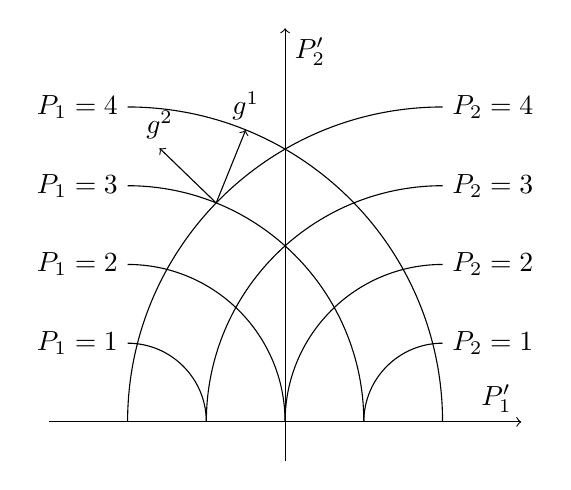
\begin{tikzpicture}
\draw[->] (-3, 0) -- (3, 0) node[anchor=south east]{\(P'_1\)};
\draw[->] (0, -0.5) -- (0, 5) node[anchor=north west]{\(P'_2\)};

\foreach \r in {1, 2, 3, 4}
	\draw[thin] (\r-2, 0) arc (0:90:\r) node[anchor=east]{\(P_1 = \r\)};

\foreach \r in {1, 2, 3, 4}
	\draw[thin] (2, \r) node[anchor=west]{\(P_2 = \r\)} arc (90:180:\r);

\draw[->] (-0.875, 2.781) -- (-0.875 + 0.375, 2.781 + 0.927) node[anchor=south]{\(\vect{g}^1\)};
\draw[->] (-0.875, 2.781) -- (-0.875 - 0.719, 2.781 + 0.695) node[anchor=south]{\(\vect{g}^2\)};
\end{tikzpicture}
 

\section{Kontravariantní vektory}

Mějme křivku \(P = \Gamma(t)\) v~souřadnicích \(P\), která je v~kartézských souřadnicích \(P'\) vyjádřena funkcí \(P' = \Gamma'(t) = p'(\Gamma_1(t), ..., \Gamma_n(t))\). Vyjádřeme první derivace souřadnic této křivky podle parametru \(t\):

\begin{equation}
\begin{split}
\frac{\partial \Gamma'_i}{\partial t} = \frac{\partial}{\partial t} p'_i(\Gamma_1(t), ..., \Gamma_n(t)) = \sum_{j=1}^n \frac{\partial p'_i}{P_j} (\Gamma_1(t), ..., \Gamma_n(t)) \cdot \frac{\partial \Gamma_j}{\partial t} = \\
\sum_{j=1}^n \frac{\partial \Gamma_j}{\partial t} \cdot \frac{\partial P'_i}{\partial P_j}
\end{split}
\end{equation}

Vidíme, že máme-li \(n\)-tici čísel \(\vect{u} = (u_1, u_2, ..., u_n) = \left( \frac{\partial \Gamma_1}{\partial t}, \frac{\partial \Gamma_2}{\partial t}, ..., \frac{\partial \Gamma_n}{\partial t} \right)\) v~soustavě souřadnic \(P\), tak ji do kartézské soustavy souřadnic \(P'\) transformujeme vztahem:

\begin{equation}
\label{eq:kontravariantni_vektor}
u'^i = \sum_{j=1}^n \frac{\partial p'_i}{\partial P_j} \cdot u^j = \sum_{j=1}^n \frac{\partial P'_i}{\partial P_j} \cdot u^j
\end{equation}

Každou \(n\)-tici čísel, která se transformuje podle vztahu \eqref{eq:kontravariantni_vektor} nazýváme kontravariantním vektorem. Všimněme si, že u~kontravariantních vektorů se index složky píše nahoře, aby se kontravariantní vektor odlišil od kovariantního. Nejedná se tedy o~umocňování, pokud bychom chtěli zapsat mocninu, pak mocněnec uzavřeme do závorky: \((u)^i\).

V~křivočarých souřadnicích tedy musíme rozlišovat 2 druhy vektorů, protože každý se transformuje jinak. To jsme v~kartézské soustavě souřadnic nemuseli.

Podívejme se na geometrický význam parciálních derivací \(\frac{\partial p'_i}{\partial P_j}\). Zaveďme označení \(\vect{g}_j = \left(\frac{\partial p'_1}{\partial P_j}, \frac{\partial p'_2}{\partial P_j}, ..., \frac{\partial p'_n}{\partial P_j}\right)\) pro vektor kontravariantní báze. Vektor \(\vect{g}_j\) tedy určuje, jak se změní kartézské souřadnice \(P'\), pokud změníme křivočarou souřadnici \(P_j\) o~velmi malou hodnotu. Má tedy směr tečny ke křivce \(p'(P_1, P_2, ..., t, ..., P_n)\) s~parametrem \(t\) na místě souřadnice \(P_j\).

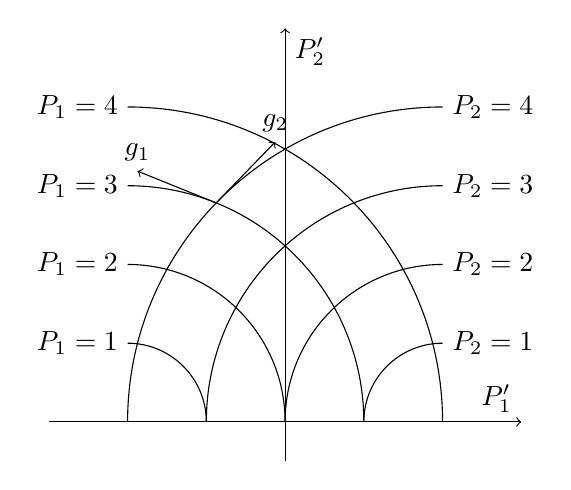
\begin{tikzpicture}
\draw[->] (-3, 0) -- (3, 0) node[anchor=south east]{\(P'_1\)};
\draw[->] (0, -0.5) -- (0, 5) node[anchor=north west]{\(P'_2\)};

\foreach \r in {1, 2, 3, 4}
	\draw[thin] (\r-2, 0) arc (0:90:\r) node[anchor=east]{\(P_1 = \r\)};

\foreach \r in {1, 2, 3, 4}
	\draw[thin] (2, \r) node[anchor=west]{\(P_2 = \r\)} arc (90:180:\r);

\draw[->] (-0.875, 2.781) -- (-0.875 - 1, 2.781 + 0.405) node[anchor=south]{\(\vect{g}_1\)};
\draw[->] (-0.875, 2.781) -- (-0.875 + 0.75, 2.781 + 0.775) node[anchor=south]{\(\vect{g}_2\)};
\end{tikzpicture}
 

\section{Tenzory}

Máme-li dva vektory, pak můžeme vytvořit součiny všech možných dvojic složek. Celkem tak získáme \(n^2\) součinů.

Začněme dvěma kovariantními vektory. Máme-li součin \(T_{ij} = u_i \cdot v_j\), pak transformovaný součin bude:

\begin{equation}
\label{eq:kovariantni_tenzor}
\begin{split}
T'_{ij} = u'_i \cdot v'_j = (\sum_{k=1}^n \frac{\partial p_k}{\partial P'_i} \cdot u_k) \cdot (\sum_{l=1}^n \frac{\partial p_l}{\partial P'_j} \cdot v_l) = \\
\sum_{k=1}^n \sum_{l=1}^n \frac{\partial p_k}{\partial P'_i} \cdot \frac{\partial p_l}{\partial P'_j} \cdot u_k \cdot v_l = \sum_{k=1}^n \sum_{l=1}^n \frac{\partial p_k}{\partial P'_i} \cdot \frac{\partial p_l}{\partial P'_j} \cdot T_{kl}
\end{split}
\end{equation}

Součin sum jsme prostě roznásobili. Například \((\sum_{i=1}^3 a_i) \cdot (\sum_{j=1}^3 b_j) = (a_1 + a_2 + a_3) \cdot (b_1 + b_2 + b_3) = a_1 b_1 + a_1 b_2 + a_1 b_3 + a_2 b_1 + a_2 b_2 + a_2 b_3 + a_3 b_1 + a_3 b_2 + a_3 b_3 = \sum_{i=1}^3 \sum_{j=1}^3 a_i b_i\). Každou veličinu \(T_{ij}\), která se transformuje podle vztahu \eqref{eq:kovariantni_tenzor}, nazýváme kovariantním tenzorem druhého řádu.

Máme-li součin dvou kontravariantních vektorů \(T^{ij} = u^i \cdot v^j\), pak transformovaný součin bude:

\begin{equation}
\label{eq:kontravariantni_tenzor}
\begin{split}
T'^{ij} = u'^i \cdot v'^j = (\sum_{k=1}^n \frac{\partial p'_i}{\partial P_k} \cdot u^k) \cdot (\sum_{l=1}^n \frac{\partial p'_j}{\partial P_l} \cdot v^l) = \\
\sum_{k=1}^n \sum_{l=1}^n \frac{\partial p'_i}{\partial P_k} \cdot \frac{\partial p'_j}{\partial P_l} \cdot u^k \cdot v^l = \sum_{k=1}^n \sum_{l=1}^n \frac{\partial p'_i}{\partial P_k} \cdot \frac{\partial p'_j}{\partial P_k} \cdot T^{kl}\end{split}
\end{equation}

Každou veličinu \(T^{ij}\), která se transformuje podle vztahu \eqref{eq:kontravariantni_tenzor}, nazýváme kontravariantním tenzorem druhého řádu.

Máme-li součin kovariantního a~kontravariantního \(T_i^j = u_i \cdot v^j\), pak transformovaný součin bude:

\begin{equation}
\label{eq:smyseny_tenzor}
\begin{split}
T'^j_i = u'_i \cdot v'^j = (\sum_{k=1}^n \frac{\partial p_k}{\partial P'_i} \cdot u_k) \cdot (\sum_{l=1}^n \frac{\partial p'_j}{\partial P_l} \cdot v^l) = \\
\sum_{k=1}^n \sum_{l=1}^n \frac{\partial p_k}{\partial P'_i} \cdot \frac{\partial p'_j}{\partial P_l} \cdot u_k \cdot v^l = \sum_{k=1}^n \sum_{l=1}^n \frac{\partial p_k}{\partial P'_i} \cdot \frac{\partial p'_j}{\partial P_l} \cdot T_k^l
\end{split}
\end{equation}

Každou veličinu \(T_i^j\), která se transformuje podle vztahu \eqref{eq:smyseny_tenzor}, nazýváme smýšeným tenzorem druhého řádu.

Vidíme, že se každý index tenzoru transformuje nezávisle na ostatních. To nám umožňuje definovat obecný tenzor:

\begin{fact}

Každou veličinu \(T_{ij...}^{kl...}\), která se transformuje podle vztahu~\eqref{eq:obecny_tenzor}, nazýváme tenzorem.

\begin{equation}
\label{eq:obecny_tenzor}
\begin{split}
T'^{kl...}_{ij...} = \sum_{s=1}^n \sum_{t=1}^n ... \sum_{u=1}^n \sum_{v=1}^n ... \frac{\partial p_s}{\partial P'_i} \cdot \frac{\partial p_t}{\partial P'_j} ... \cdot \frac{\partial p'_k}{\partial P_u} \cdot \frac{\partial p'_l}{\partial P_v} ... \cdot T_{st...}^{uv...} = \\
\tau_{P}^{P'} (T_{st...}^{uv...})
\end{split}
\end{equation}

\end{fact}

Počet indexů určuje řád tenzoru. Tenzor nultého řádu je skalár. Tenzor prvního řádu je kovariantní nebo kontravariantní vektor.

Zavedli jsme označení \(\tau_{P}^{P'}\) pro transformaci tenzoru ze souřadného systému \(P\) do souřadného systému \(P'\). Upozorňuji, že tato transformace není funkce, nepracuje s~jednou složkou tenzoru, ale s~celým tenzorem. Zavedli jsme ji pro zjednodušení zápisu. Povšimněme si, že tato transformace je lineárním tedy:

\begin{equation}
\label{eq:linearni_transformace_tenzoru}
\begin{split}
\alpha \cdot \tau_{P}^{P'}(S_{st...}^{uv...}) + \beta \cdot \tau_{P}^{P'}(T_{st...}^{uv...})) = \tau_{P}^{P'}(\alpha \cdot S_{st...}^{uv...} + \beta \cdot T_{st...}^{uv...})
\end{split}
\end{equation}

\section{Operace s~tenzory}

Prozkoumejme operace, které lze s~tenzory provádět. V~kapitole o~Euklidovském prostoru jsme operace sčítání a~násobení vektorů odvodili geometricky. V~křivočarých souřadnicích však rozdíl souřadnic dvou bodů obecně není vektor, operace s~vektory ani tenzory proto nemůžeme zavést geometricky. Můžeme je však zavést transformací do Euklidovského prostoru.

Víme, že v~Euklidovském prostoru je vztah mezi vektory a~jejich složkami lineární. Tedy že vektor \(\vect{w} = \alpha \cdot \vect{u} + \beta \cdot \vect{v}\) má složky \(w_i = \alpha \cdot u_i + \beta \cdot v_i\). Transformace \(\tau\) je lineární, takže pokud bychom soustavu souřadnic \(P\) zvolili za Euklidovskou, tak i~soustavě souřadnic \(P'\) bude platit lineární vztah mezi vektory a~jeho složkami. Pro skaláry uvedený vztah samozřejmě platí taky. Je tedy celkem přirozené, když linearitu rozšíříme na obecný tenzor:

\begin{equation}
\label{eq:scitani_a_nasobeni_tenzoru}
\begin{split}
U = \alpha \cdot S + \beta \cdot T \Leftrightarrow U_{st...}^{uv...} = \alpha \cdot S_{st...}^{uv...} + \beta \cdot T_{st...}^{uv...}
\end{split}
\end{equation}

Sčítat můžeme pouze tenzory stejného druhu, tedy tenzory se stejným počtem kovariantních a~kontravariantních indexů. Násobení tenzorů skalárem a~dříve popsané složkové násobení vektorů můžeme zobecnit na násobení dvou tenzorů. Vytvoříme součiny všech dvojic složek tenzorů:

\begin{equation}
\label{eq:nasobeni_tenzoru}
U = S \otimes T \Leftrightarrow U_{st...}^{uv...} = S_{s...}^{u...} \cdot T_{t...}^{v...}
\end{equation}

Prozkoumejme, jak se bude tento součin transformovat.

\begin{equation}
\begin{split}
U'^{kl...}_{ij...} = \tau_{P}^{P'}(S_{s...}^{u...}) \cdot \tau_{P}^{P'}(T_{t...}^{v...}) = \\
\left( \sum_{s=1}^n ... \sum_{u=1}^n ... \frac{\partial p_s}{\partial P'_i} ... \cdot \frac{\partial p'_k}{\partial P_u} ... \cdot T_{s...}^{u...} \right) \cdot \left( \sum_{t=1}^n ... \sum_{v=1}^n ... \frac{\partial p_t}{\partial P'_j} ... \cdot \frac{\partial p'_l}{\partial P_v} ... \cdot T_{t...}^{v...} \right) = \\
\sum_{s=1}^n \sum_{t=1}^n ... \sum_{u=1}^n \sum_{v=1}^n ... \frac{\partial p_s}{\partial P'_i} \cdot \frac{\partial p_t}{\partial P'_j} ... \cdot \frac{\partial p'_k}{\partial P_u} \cdot \frac{\partial p'_l}{\partial P_v} ... \cdot T_{s...}^{u...} \cdot T_{t...}^{v...} = \\
\tau_{P}^{P'}(T_{s...}^{u...} \cdot T_{t...}^{v...})
\end{split}
\end{equation}

Vidíme, že se součin tenzorů transformuje jako tenzor a~je tedy tenzorem s~počtem kovariantních indexů rovným součtu počtu kovariantních indexů součinitelů a~s~počtem kontravariantních indexů rovným součtu počtu kontravariantních indexů součinitelů. 

\section{Zůžení tenzoru}

V~Euklidovském prostoru jsme zavedli skalární součin vektorů. Něco obdobného bychom chtěli zavést i~v~křivočarých souřadnicích. Nejdříve však musíme vyjádřit vztah mezi derivacemi souřadnic.

Začněme tím, že vyjádříme reverzibilitu transformace souřadnic. Souřadnice \(P_i\) považujme za závislé na parametru \(t\), \(P\) tedy bude křivka.

\begin{equation}
p_k(p'_1(P_1(t), ..., P_n(t)), ..., p'_n(P_1(t), ..., P_n(t))) = P_k(t)
\end{equation}

Zderivujme rovnici podle parametru \(t\):

\begin{equation}
\label{eq:reverzibilni_derivace}
\sum_{i=1}^n \frac{\partial p_k}{\partial P'_i} \cdot \sum_{j=1}^n \frac{\partial p'_i}{\partial P_j} \cdot \frac{\partial P_j}{\partial t} = \frac{\partial P_k}{\partial t}
\end{equation}

Tato soustava rovnic musí platit pro jakoukoli sadu funkcí \(P_j\), která má definované první derivace. Zvolme tedy jednu konkrétní sadu: \(P_1 = t\), \(P_2, P_3, ..., P_n = 0\) a~vyjádřeme rovnici~\eqref{eq:reverzibilni_derivace} pro \(k = 1\):

\begin{equation}
\sum_{i=1}^n \frac{\partial p_1}{\partial P'_i} \frac{\partial p'_i}{\partial P_1} = 1
\end{equation}

Ve vnitřní sumě jsou všechny členy nulové kromě členu \(j = 1\), sumu jsme proto nahradili tímto jedním členem.
Dále vyjádřeme rovnici~\eqref{eq:reverzibilni_derivace} pro \(k = 2\):

\begin{equation}
\sum_{i=1}^n \frac{\partial p_2}{\partial P'_i} \frac{\partial p'_i}{\partial P_1} = 0
\end{equation}

Obdobně budeme postupovat pro ostatní \(k\).

Zvolme dále sadu funkcí: \(P_1 = 0\), \(P_2 = t\), \(P_3, P_4, ..., P_n = 0\) a~vyjádřeme rovnici~\eqref{eq:reverzibilni_derivace} pro \(k = 1\):

\begin{equation}
\sum_{i=1}^n \frac{\partial p_1}{\partial P'_i} \frac{\partial p'_i}{\partial P_2} = 0
\end{equation}

Pro \(k = 2\) obdržíme

\begin{equation}
\sum_{i=1}^n \frac{\partial p_2}{\partial P'_i} \frac{\partial p'_i}{\partial P_2} = 1
\end{equation}

Vidíme, že obecně pro libovolné \(k\) a~\(j\) musí platit:

\begin{equation}
\sum_{i=1}^n \frac{\partial p_k}{\partial P'_i} \frac{\partial p'_i}{\partial P_j} =
\begin{cases}
	1 \text{ pokud } k = j \\
	0 \text{ pokud } k \neq j
\end{cases}
\end{equation}

Celý výpočet si můžeme zjednodušit, pokud zavedeme Kroneckerův symbol delta:

\begin{equation}
\delta_{ij} =
\begin{cases}
	1 \text{ pokud } i = j \\
	0 \text{ pokud } i \neq j
\end{cases}
\end{equation}

Sadu funkcí \(P\) definujeme \(P_j = \delta_{jl} \cdot t\) pro zvolený parametr \(l\). Dosazením do rovnice~\eqref{eq:reverzibilni_derivace} získáme:

\begin{equation}
\label{eq:vztah_mezi_bazemi}
\begin{split}
\sum_{i=1}^n \frac{\partial p_k}{\partial P'_i} \cdot \sum_{j=1}^n \frac{\partial p'_i}{\partial P_j} \cdot \delta_{jl} = \delta_{kl} \\
\sum_{i=1}^n \frac{\partial p_k}{\partial P'_i} \cdot \frac{\partial p'_i}{\partial P_l} = \delta_{kl}
\end{split}
\end{equation}

Opět jsme nahradili vnitřní sumu jejím jediným nenulovým prvkem. Nyní můžeme přistoupit k~formulaci zúžení tenzoru. 

\begin{fact}
Mějme tenzor \(T_{ij...}^{kl...}\) s~libovolným kovariantním indexem \(i\) a~libovolným kontravariantním indexem \(k\). Pak \(S_{j...}^{l...} = \sum_{i=1}^n T_{ij...}^{il...}\) je tenzor.
\end{fact}

Při zúžení tenzoru tedy vybereme jeden kovariantní a~jeden kontravariantní index a~sečteme složky tenzoru, ve kterých jsou tyto indexy shodné. Získáme tak tenzor o~2 řády nižší.

Dokažme, že získaná veličina je opravdu tenzor tím, že prozkoumáme, jak se transformuje:

\begin{equation}
\begin{split}
T'^{kl...}_{ij...} = \tau_P^{P'} (T_{st...}^{uv...}) = \\
\sum_{s=1}^n \sum_{t=1}^n ... \sum_{u=1}^n \sum_{v=1}^n ... \frac{\partial p_s}{\partial P'_i} \cdot \frac{\partial p_t}{\partial P'_j} ... \cdot \frac{\partial p'_k}{\partial P_u} \cdot \frac{\partial p'_l}{\partial P_v} ... \cdot T_{st...}^{uv...}
\end{split}
\end{equation}

\begin{equation}
\begin{split}
S_{t...}^{v...} = \sum_{w=1}^n T_{wt...}^{wv...}
\end{split}
\end{equation}

\begin{equation}
\begin{split}
S'^{l...}_{j...} = \sum_{w=1}^n T'^{wl...}_{wj...} = \\
\sum_{w=1}^n \sum_{s=1}^n \sum_{t=1}^n ... \sum_{u=1}^n \sum_{v=1}^n ... \frac{\partial p_s}{\partial P'_w} \cdot \frac{\partial p_t}{\partial P'_j} ... \cdot \frac{\partial p'_w}{\partial P_u} \cdot \frac{\partial p'_l}{\partial P_v} ... \cdot T_{st...}^{uv...} = \\
\sum_{s=1}^n \sum_{t=1}^n ... \sum_{u=1}^n \sum_{v=1}^n ... \frac{\partial p_t}{\partial P'_j} ... \cdot \frac{\partial p'_l}{\partial P_v} ... \cdot T_{st...}^{uv...} \cdot \sum_{w=1}^n \frac{\partial p_s}{\partial P'_w} \cdot \frac{\partial p'_w}{\partial P_u} = \\
\sum_{s=1}^n \sum_{t=1}^n ... \sum_{u=1}^n \sum_{v=1}^n ... \frac{\partial p_t}{\partial P'_j} ... \cdot \frac{\partial p'_l}{\partial P_v} ... \cdot T_{st...}^{uv...} \cdot \delta_{su} = \\
\sum_{w=1}^n \sum_{t=1}^n ... \sum_{v=1}^n ... \frac{\partial p_t}{\partial P'_j} ... \cdot \frac{\partial p'_l}{\partial P_v} ... \cdot T_{wt...}^{wv...} = \\
\sum_{t=1}^n ... \sum_{v=1}^n ... \frac{\partial p_t}{\partial P'_j} ... \cdot \frac{\partial p'_l}{\partial P_v} ... \cdot S_{t...}^{v...} = \\
\tau_P^{P'} (S_{t...}^{v...})
\end{split}
\end{equation}

Pokud bychom chtěli sčítat přes dva kovariantní nebo dva kontravariantní indexy, tak by se výsledek netransformoval jako tenzor. Takovéto zůžení tedy nebudeme
vůbec uvažovat.

Zůžení nám umožňuje definovat skalární součin kovariantního a~kontravariantního vektoru jako zůžení tenzorového součinu těchto vektorů. Zavedeme při tom
konvenci, že vektor s~šipkou nad symbolem bude kontravariantní a~vektor s~šipkou pod symbolem bude kovaraintní. Pozice šipky tak bude shodná s~pozicí
indexu ve složkovém zápisu. Dále šipka nad vektorem bude odpovídat vektoru mezi dvěma body, který je také kontravariantní.

\begin{fact}
Skalární součin \(s = \kovarvect{u} \cdot \kontravect{v}\) vypočítáme podle vztahu \(s = \sum_{i=1}^n u_i \cdot v^i\).
\end{fact}

\section{Délka, obsah, objem}

Předpokládejme, že \(P'\) je kartézský systém souřadnic. Mějme kontravariatní vektor \(\kontravect{v'}\). Pak jeho délka bude

\begin{equation}
l = \sqrt{\sum_{i=1}^n (v'^i)^2}
\end{equation}

V~souřadném systému \(P\) bude délka vektoru \(\kontravect{v}\)

\begin{equation}
\begin{split}
l = \sqrt{\sum_{i=1}^n \left(\sum_{j=1}^n \frac{\partial p'_i}{\partial P_j} v^j \right)^2} = \sqrt{\sum_{i=1}^n \sum_{j=1}^n \sum_{k=1}^n \frac{\partial p'_i}{\partial P_j} \frac{\partial p'_i}{\partial P_k} v^j v^k} = \\
\sqrt{\sum_{j=1}^n \sum_{k=1}^n v^j v^k \sum_{i=1}^n \frac{\partial p'_i}{\partial P_j} \frac{\partial p'_i}{\partial P_k}} = \sqrt{\sum_{j=1}^n \sum_{k=1}^n g_{jk} v^j v^k}
\end{split}
\end{equation}

Zavedli jsme označení \(g_{jk} = \sum_{i=1}^n \frac{\partial p'_i}{\partial P_j} \frac{\partial p'_i}{\partial P_k} = \vect{g}_j \cdot \vect{g}_k\). Délka \(l\) je invariantní vůči změně souřadného systému. Je tedy zřejmé, že \(g_{jk}\) musí být kovariantním tenzorem druhého řádu. Jedná se o~tenzor symetrický, tedy \(g_{jk} = g_{kj}\). Nazýváme jej kovariantním metrickým tenzorem. Číselně je hodnota \(g_{jk}\) rovna skalárnímu součinu vektoru báze \(\vect{g}_j\) s~vektorem báze \(\vect{g}_k\).

Všimněme si, že vztah se velmi zjednoduší, pokud \(g_{jk} = 0\) pro \(j \neq k\):

\begin{equation}
l = \sqrt{\sum_{i=1}^n g_{ii} (v^i)^2}
\end{equation}

Vztah nám velmi připomíná rovnici~\eqref{eq:vektor_velikost}, pouze druhé mocniny složek vektoru jsou váženy vahami \(g_{ii}\). Speciálně pro diferenciály souřadnic platí:

\begin{equation}
\label{eq:delka_diferencial_souradnic}
dl = g_{ii} dx_i
\end{equation}

Tento vztah můžeme využít pro integrování podél souřadnicové osy.

Povšimněme si, že \(g_{jk}\) je pro \(j \neq k\) nulový právě tehdy, pokud jsou vektory báze \(\vect{g}_i\) vzájemně kolmé. Takovémuto souřadnému systému říkáme ortogonální. Celá řada souřadnicových systémů jsou ortogonální - například kartézský, polární, cylindrický i~sférický. Proto má smysl se jimi zabývat.

Přejděme dále k~obsahu. Mějme 2 diferenciály souřadnic \(dx_i\) a~\(dx_j\), \(i \neq j\). Potom v~ortogonálním systému souřadnic bude platit:

\begin{equation}
\label{eq:obsah_diferencial_souradnic}
dS = g_{ii} g_{jj} dx_i dx_j
\end{equation}

Vztah \eqref{eq:obsah_diferencial_souradnic} jsme odvodili jako obsah obdélníka, jehož strany jsou určeny vztahem~\eqref{eq:delka_diferencial_souradnic}. Využíváme při tom faktu, že souřadnicové osy jsou na sebe kolmé.

Obdobně můžeme vypočítat objem kvádru se stranami určenými diferenciály souřadnic \(dx_i\), \(dx_j\) a~\(dx_k\):

\begin{equation}
\label{eq:objem_diferencial_souradnic}
dV = g_{ii} g_{jj} g_{kk} dx_i dx_j dx_k
\end{equation}

Obdobně můžeme vypočítat délku kovariantního vektoru:

\begin{equation}
\begin{split}
l = \sqrt{\sum_{i=1}^n \left(\sum_{j=1}^n \frac{\partial p_j}{\partial P'_i} v_j \right)^2} = \sqrt{\sum_{i=1}^n \sum_{j=1}^n \sum_{k=1}^n \frac{\partial p_j}{\partial P'_i} \cdot \frac{\partial p_k}{\partial P'_i} v_j v_k} = \\
\sqrt{\sum_{j=1}^n \sum_{k=1}^n v_j v_k \sum_{i=1}^n} \frac{\partial p_j}{\partial P'_i} \frac{\partial p_k}{\partial P'_i} = \sqrt{\sum_{j=1}^n \sum_{k=1}^n g^{jk} v_j v_k}
\end{split}
\end{equation}

Veličinu \(g^{jk} = \sum_{i=1}^n \frac{\partial p_j}{\partial P'_i} \frac{\partial p_k}{\partial P'_i}\) nazveme kontravariantním metrickým tenzorem. Opět se jedná o~symetrický tenzor druhého řádu.


\section{Zpětná transformace}

Doposud jsme řešili, jak se transformují veličiny z~křivočaré soustavy souřadnic \(P\) do kartézské soustavy souřadnic \(P'\). Nyní prozkoumáme transformaci opačnou - z~kartézské soustavy souřadnic \(P\) do křivočaré soustavy souřadnic \(P'\).
Vraťme se k~rovnici \eqref{eq:vztah_mezi_bazemi}, vynásobme ji kontravariantním vektorem \(v^l\) a~proveďme sumaci přes index \(l\):
 
\begin{equation}
\label{eq:transformace_kontravariantniho_vektoru_z_kartezske_soustavy}
\begin{split}
\sum_{i=1}^n \frac{\partial p_k}{\partial P'_i} \cdot \frac{\partial p'_i}{\partial P_l} = \delta_{kl} \\
\sum_{i=1}^n \frac{\partial p_k}{\partial P'_i} \cdot \frac{\partial p'_i}{\partial P_l} v^l = \delta_{kl} \cdot v^l \\
\sum_{l=1}^n \sum_{i=1}^n \frac{\partial p_k}{\partial P'_i} \cdot \frac{\partial p'_i}{\partial P_l} v^l = \sum_{l=1}^n \delta_{kl} \cdot v^l \\
\sum_{i=1}^n \frac{\partial p_k}{\partial P'_i} \cdot \sum_{l=1}^n \frac{\partial p'_i}{\partial P_l} v^l = v^k \\
\sum_{i=1}^n \frac{\partial p_k}{\partial P'_i} v'^i = v^k
\end{split}
\end{equation}

Vidíme, že kontravariantní vektor se transformuje z~kartézské do křivočaré soustavy souřadnic jako kovariantní vektor opačným směrem. To není překvapivé uvážíme-li, že transformační funkce \(p_i\) a \(p'_i\) jsou vzájemně inverzní. Obdobně se kovariantní vektor transformuje z~kartézské do křivočaré soustavy souřadnic jako kontravariantní vektor opačným směrem:

\begin{equation}
\label{eq:transformace_kovariantniho_vektoru_z_kartezske_soustavy}
\begin{split}
\sum_{i=1}^n \frac{\partial p'_i}{\partial P_l} \cdot \frac{\partial p_k}{\partial P'_i} = \delta_{kl} \\
\sum_{i=1}^n \frac{\partial p'_i}{\partial P_l} \cdot \frac{\partial p_k}{\partial P'_i} v_k = \delta_{kl} \cdot v_k \\
\sum_{k=1}^n \sum_{i=1}^n \frac{\partial p'_i}{\partial P_l} \cdot \frac{\partial p_k}{\partial P'_i} v_k = \sum_{k=1}^n \delta_{kl} \cdot v_k \\
\sum_{i=1}^n \frac{\partial p'_i}{\partial P_l} \cdot \sum_{k=1}^n \frac{\partial p_k}{\partial P'_i} v_k = v_l \\
\sum_{i=1}^n \frac{\partial p'_i}{\partial P_l} \cdot v'_i = v_l \\
\end{split}
\end{equation}

Obdobně můžeme transformovat i~tenzory, pro každý index provedeme tuto transformaci zvlášť.

V~kartézské soustavě souřadnic ale nemusíme rozlišovat mezi kovariantními a~kontravariantními vektory, přesněji jejich složky jsou shodné. S~využitím rovnice~\eqref{eq:transformace_kovariantniho_vektoru_z_kartezske_soustavy} tak můžeme definovat transformaci kontravariantního vektoru na kovariantní tak, že kontravariantní vektor transformujeme do kartézské soustavy souřadnic a~z~té ho jako kovaraintní vektor transformujeme zpět do křivočaré soustavy souřadnic:

\begin{equation}
\begin{split}
v_l = \sum_{i=1}^n \frac{\partial p'_i}{\partial P_l} \cdot v'_i = \sum_{i=1}^n \frac{\partial p'_i}{\partial P_l} \cdot \sum_{j=1}^n \frac{\partial p'_i}{\partial P_j} v^j = \sum_{j=1}^n \sum_{i=1}^n \frac{\partial p'_i}{\partial P_l} \frac{\partial p'_i}{\partial P_j} v^j = \sum_{j=1}^n g_{lj} v^j
\end{split}
\end{equation}

Kontravariantní tenzor tedy transformujeme na kovariantní tak, že jej vynásobíme kovariantním metrickým tenzorem a~zůžíme jej (podle libovolného indexu - metrický tenzor je symetrický). Této operaci říkáme snižování indexu a~lze ji provádět pro libovolný kontravariantní index tenzoru.

Obdobně můžeme s~pomocí rovnice~\eqref{eq:transformace_kontravariantniho_vektoru_z_kartezske_soustavy} definovat transformaci kovariantního vektoru na kontravariantní:

\begin{equation}
\begin{split}
v^k = \sum_{i=1}^n \frac{\partial p_k}{\partial P'_i} v'^i = \sum_{i=1}^n \frac{\partial p_k}{\partial P'_i} \cdot \sum_{j=1}^n \frac{\partial p_j}{\partial P'_i} v_j = \sum_{j=1}^n \sum_{i=1}^n \frac{\partial p_k}{\partial P'_i} \frac{\partial p_j}{\partial P'_i} v_j = \sum_{j=1}^n g^{jk} v_j
\end{split}
\end{equation}

Vidíme, že kovariantní a~kontravariantní vektory lze mezi sebou převádět. Můžeme tedy hovořit o~vektoru \(\vect{v}\), který má kovariantní složky \(v_i\) a~kontravariantní složky \(v^i\). Této operaci říkáme zvedání indexu a~lze ji provádět pro libovolný kovariantní index tenzoru.

\section{Vyjádření některých operací}

Umíme-li provádět transformace vektorů, tak můžeme vyjádřit operace s~vektory v~křivočarých souřadnicích. 

\subsection{Skalární součin}

Začněme skalárním součinem vektorů \(\vect{u} \cdot \vect{v}\). Už víme, jak vypočítat skalární součin kovariantního a~kontravariantního vektoru. Transformací jednoho vektoru pak můžeme vypočítat skalární součin dvou vektorů stejného druhu:

\begin{fact}
\begin{equation}
\begin{split}
\kovarvect{u} \cdot \kontravect{v} = \sum_{i=1}^n u_i \cdot v^i \\
\kovarvect{u} \cdot \kovarvect{v} = \sum_{i=1}^n \sum_{j=1}^n u_i \cdot v_i \cdot g^{ij} \\
\kontravect{u} \cdot \kontravect{v} = \sum_{i=1}^n \sum_{j=1}^n u^i \cdot v^i \cdot g_{ij}
\end{split}
\end{equation}
\end{fact}

\subsection{Levi-Civitův symbol}

Podívejme se, jak se transformuje Levi-Civitův symbol do křivočarých souřadnic. Levi-Civitův symbol je kartézským tenzorem, můžeme jej proto transformovat na kovariantní i~kontravariantní tenzor v křivočarých souřadnicích, kde jej budeme značit \(\epsilon_{ijk}\) potažmo \(\epsilon^{ijk}\).

Začněme transformací na kovariantní tenzor. 

\begin{equation}
\begin{split}
\epsilon_{lmn} = \sum_{i=1}^3 \sum_{j=1}^3 \sum_{k=1}^3 \frac{\partial p'_i}{\partial P_l} \frac{\partial p'_j}{\partial P_m} \frac{\partial p'_k}{\partial P_n} \cdot \varepsilon_{ijk}
\end{split}
\end{equation}

Prozkoumejme, pro které indexy \(lmn\) získáme nenulové \(\epsilon_{lmn}\). Začněme situací, kdy máme 2 indexy stejné. Nechť jsou to například indexy \(l = m\). Pak

\begin{equation}
\begin{split}
\epsilon_{lln} = \sum_{i=1}^3 \sum_{j=1}^3 \sum_{k=1}^3 \frac{\partial p'_i}{\partial P_l} \frac{\partial p'_j}{\partial P_l} \frac{\partial p'_k}{\partial P_n} \cdot \varepsilon_{ijk}
\end{split}
\end{equation}

Součet členů jde přes všechny permutace indexů \(i\), \(j\) a \(k\). Proto se budou členy \(\frac{\partial p'_i}{\partial P_l} \frac{\partial p'_j}{\partial P_l} \frac{\partial p'_k}{\partial P_n}\) v~součtu vyskytovat po dvojicích s~prohozenými indexy \(i\) a \(j\). Tyto dvojice budou odpovídat sudé a~liché permutaci indexů \(i\), \(j\) a \(k\), proto symbol \(\varepsilon_{ijk}\) bude mít opačné znaménko a~všechny členy se v~součtu vyruší. Tenzor \(\epsilon_{lmn}\) proto bude mít nenulové prvky jen pro různé indexy \(l\), \(m\) a~\(n\).

Vyšetřeme tedy tenzor \(\epsilon_{lmn}\) pro různé indexy \(l\), \(m\) a~\(n\). Uvědomme si, že v~členech \(\frac{\partial p'_i}{\partial P_l} \frac{\partial p'_j}{\partial P_m} \frac{\partial p'_k}{\partial P_n}\) můžeme jednotlivé součinitele libovolně prohazovat beze změny jejich hodnot. Sou4initele proto můžeme přeskládat tak, aby členy byly ve tvaru \(\frac{\partial p'_a}{\partial P_1} \frac{\partial p'_b}{\partial P_2} \frac{\partial p'_c}{\partial P_3}\). Pokud posloupnost \([l, m, n]\) představovala sudou permutaci posloupnosti \([1, 2, 3]\), pak je potřeba sudý počet prohození součinitelů, pokud představovala permutaci lichou, pak je potřeba lichý počet prohození součinitelů. Spolu s~tím dochází ale i~k permutaci posloupností \([i, j, k]\) na posloupnosti \([a, b, c]\). Protože provádíme součet přes všechny permutace, tak budeme sčítat všechny členy i~po přeskládání součinitelů, ale při lichém počtu prohození součinitelů, tedy pokud je permutace \([l, m, n]\) lichá, je nutné násobit součinitele číslem -1. To přesně odpovídá Levi-Civitově symbolu:

\begin{equation}
\begin{split}
\epsilon_{lmn} = \left(\sum_{i=1}^3 \sum_{j=1}^3 \sum_{k=1}^3 \frac{\partial p'_i}{\partial P_1} \frac{\partial p'_j}{\partial P_2} \frac{\partial p'_k}{\partial P_3} \cdot \varepsilon_{ijk} \right) \cdot \varepsilon_{lmn} = \\
\begin{vmatrix}
  \frac{\partial p'_1}{\partial P_1} & \frac{\partial p'_2}{\partial P_1} & \frac{\partial p'_3}{\partial P_1} \\
  \frac{\partial p'_1}{\partial P_2} & \frac{\partial p'_2}{\partial P_2} & \frac{\partial p'_3}{\partial P_2} \\
  \frac{\partial p'_1}{\partial P_3} & \frac{\partial p'_2}{\partial P_3} & \frac{\partial p'_3}{\partial P_3}
\end{vmatrix}
\cdot \varepsilon_{lmn} = J \cdot \varepsilon_{lmn}
\end{split}
\end{equation}

Vidíme, že Levi-Civitův symbol se transformuje pouze násobením konstantou, tzv. Jakobiánem funkcí \(p'_i\), pro nějž jsme zavedli označení:

\begin{equation}
J = 
\begin{vmatrix}
  \frac{\partial p'_1}{\partial P_1} & \frac{\partial p'_2}{\partial P_1} & \frac{\partial p'_3}{\partial P_1} \\
  \frac{\partial p'_1}{\partial P_2} & \frac{\partial p'_2}{\partial P_2} & \frac{\partial p'_3}{\partial P_2} \\
  \frac{\partial p'_1}{\partial P_3} & \frac{\partial p'_2}{\partial P_3} & \frac{\partial p'_3}{\partial P_3}
\end{vmatrix}
\end{equation}

Obdobně můžeme transformovat Levi-Civitův symbol na kontravariantní tenzor:

\begin{equation}
\begin{split}
\epsilon^{lmn} = \sum_{i=1}^3 \sum_{j=1}^3 \sum_{k=1}^3 \frac{\partial p_l}{\partial P'_i} \frac{\partial p_m}{\partial P'_j} \frac{\partial p_n}{\partial P'_k} \cdot \varepsilon_{ijk} = \\
\left(\sum_{i=1}^3 \sum_{j=1}^3 \sum_{k=1}^3 \frac{\partial p_1}{\partial P'_i} \frac{\partial p_2}{\partial P'_j} \frac{\partial p_3}{\partial P'_k} \cdot \varepsilon_{ijk} \right) \cdot \varepsilon_{lmn} = \\
\begin{vmatrix}
  \frac{\partial p_1}{\partial P'_1} & \frac{\partial p_2}{\partial P'_1} & \frac{\partial p_3}{\partial P'_1} \\
  \frac{\partial p_1}{\partial P'_2} & \frac{\partial p_2}{\partial P'_2} & \frac{\partial p_3}{\partial P'_2} \\
  \frac{\partial p_1}{\partial P'_3} & \frac{\partial p_2}{\partial P'_3} & \frac{\partial p_3}{\partial P'_3}
\end{vmatrix}
\cdot \varepsilon_{lmn}  = J' \cdot \varepsilon_{lmn}
\end{split}
\end{equation}

Vidíme, že Levi-Civitův symbol se transformuje pouze násobením konstantou, tzv. Jakobiánem funkcí \(p_i\), pro nějž jsme zavedli označení:

\begin{equation}
J' = \begin{vmatrix}
  \frac{\partial p_1}{\partial P'_1} & \frac{\partial p_2}{\partial P'_1} & \frac{\partial p_3}{\partial P'_1} \\
  \frac{\partial p_1}{\partial P'_2} & \frac{\partial p_2}{\partial P'_2} & \frac{\partial p_3}{\partial P'_2} \\
  \frac{\partial p_1}{\partial P'_3} & \frac{\partial p_2}{\partial P'_3} & \frac{\partial p_3}{\partial P'_3}
\end{vmatrix}
\end{equation}

\subsection{Vektorový součin}

Prozkoumejme, jak se transformuje vektorový součin. Pro kartézské vektory platí rovnice \eqref{eq:vektorovy_soucin}, pro názornost si ji znovu připomeneme:

\begin{equation}
\begin{split}
\vect{v} = \vect{b} \times \vect{c} \\
v_i = \sum_{j=1}^3 \sum_{k=1}^3 b_j c_k \varepsilon_{ijk}
\end{split}
\end{equation}

Vidíme, že rovnice má tvar dvojího zůžení součinu vektorů \(b_j\), \(c_k\) a~tenzoru \(\varepsilon_{ijk}\). To nám umožňuje přímo zapsat vektorový součin dvou kovariantních a~dvou kontravariantních vektorů:

\begin{equation}
v^i = \sum_{j=1}^3 \sum_{k=1}^3 b_j c_k \epsilon^{ijk}
\end{equation}

\begin{equation}
v_i = \sum_{j=1}^3 \sum_{k=1}^3 b^j c^k \epsilon_{ijk}
\end{equation}

\subsection{Derivace vektorů}

Mějme derivaci soužky kartézského vektoru \(u_i\) podle souřadnice \(j\). Vyjádřeme ji pro kovariantní vektor:

\begin{equation}
\label{eq:derivace_vektoru}
\begin{split}
\frac{\partial u'_i}{\partial P'_j} = \frac{\partial}{\partial P'_j} \sum_{k=1}^n \frac{\partial p_k}{\partial P'_i} \cdot u_k \\
\frac{\partial}{\partial P'_j} \sum_{k=1}^n \frac{\partial p_k}{\partial P'_i}(P'_1, ..., P'_n) \cdot u_k(p_1(P'_1, ..., P'_n), ..., p_n(P'_1, ..., P'_n)) = \\
\sum_{k=1}^n \frac{\partial}{\partial P'_j} \left( \frac{\partial p_k}{\partial P'_i}(P'_1, ..., P'_n) \cdot u_k(p_1(P'_1, ..., P'_n), ..., p_n(P'_1, ..., P'_n)) \right) = \\
\sum_{k=1}^n \left(\frac{\partial p_k}{\partial P'_i} \sum_{l=1}^n \frac{\partial u_k}{\partial P_l} \cdot \frac{\partial p_l}{\partial P'_j} + \frac{\partial^2 p_k}{\partial P'_i P'_j} \cdot u_k \right) = \\
\sum_{k=1}^n \sum_{l=1}^n \frac{\partial p_k}{\partial P'_i} \frac{\partial p_l}{\partial P'_j} \frac{\partial u_k}{\partial P_l} + \sum_{k=1}^n \frac{\partial^2 p_k}{\partial P'_i P'_j} u_k
\end{split} 
\end{equation}

Vidíme, že derivace v~křivočarých souřadnicích sestává ze dvou členů. První člen odpovídá transformaci tenzoru, druhý člen odpovídá zakřivení souřadného systému. Tento druhý člen způsobuje, že derivace vektoru obecně není tenzor. Pokud ale uděláme rozdíl \(\frac{\partial u'_i}{\partial P'_j} - \frac{\partial u'_j}{\partial P'_i}\), tak se tento druhý člen vyruší a~tento rozdíl je tenzorem druhého řádu:

\begin{equation}
\label{eq:tenzor_rozdil_derivaci_vektoru}
\frac{\partial u'_i}{\partial P'_j} - \frac{\partial u'_j}{\partial P'_i} =
\sum_{k=1}^n \sum_{l=1}^n \frac{\partial p_k}{\partial P'_i} \frac{\partial p_l}{\partial P'_j} \left(\frac{\partial u_k}{\partial P_l} - \frac{\partial u_l}{\partial P_k} \right) 
\end{equation}
